\documentclass{beamer}
\usepackage{algorithm} %pseudo-code
\usepackage{algpseudocode}
\usepackage{amsmath, amssymb, amscd}
\usepackage{graphicx}
\usepackage{float}
\usepackage{amsmath, amssymb, amscd}
\usepackage{alltt}
\usepackage{textcomp}
\usepackage{gensymb}
\usepackage{multicol}
\usepackage{tabularx}

\newcommand{\N}{\mathbb{N}}
\newcommand{\Z}{\mathbb{Z}}
\newcommand{\R}{\mathbb{R}}
\newcommand{\bigo}{\mathcal{O}}
\newcommand{\G}{\mathcal{G}}
\newcommand{\V}{\mathcal{V}}
\newcommand{\E}{\mathcal{E}}
\newcommand{\K}{\mathcal{K}}
\newcommand{\T}{^\intercal}

\newcommand{\sups}[1]{\ensuremath{^{\textrm{#1}}}}
\newcommand{\subs}[1]{\ensuremath{_{\textrm{#1}}}}

\newcommand{\specialcell}[2][c]
{
  \begin{tabular}[#1]{@{}c@{}}#2\end{tabular}
}

\makeatletter
\newsavebox{\mybox}\newsavebox{\mysim}
\newcommand{\distras}[1]
{
  \savebox{\mybox}{\hbox{\kern3pt$\scriptstyle#1$\kern3pt}}%
  \savebox{\mysim}{\hbox{$\sim$}}%
  \mathbin{\overset{#1}{\kern\z@\resizebox{\wd\mybox}{\ht\mysim}{$\sim$}}}%
}
\makeatother
%===============================================================================
% code highlighting :
\usepackage{listings}

% define custom colors :
\usepackage{color}
\definecolor{bg}{rgb}{0.96,0.96,0.85}
\definecolor{deepblue}{rgb}{0,0,0.5}
\definecolor{deepred}{rgb}{0.6,0,0}
\definecolor{deepgreen}{rgb}{0,0.5,0}

\usepackage{xcolor}
\renewcommand{\lstlistlistingname}{Code Listings}
\renewcommand{\lstlistingname}{Code Listing}
\definecolor{gray}{gray}{0.5}
\colorlet{commentcolour}{green!50!black}

\colorlet{stringcolour}{red!60!black}
\colorlet{keywordcolour}{magenta!90!black}
\colorlet{exceptioncolour}{yellow!50!red}
\colorlet{commandcolour}{blue!60!black}
\colorlet{numpycolour}{blue!60!green}
\colorlet{literatecolour}{magenta!90!black}
\colorlet{promptcolour}{green!50!black}
\colorlet{specmethodcolour}{violet}
\colorlet{indendifiercolour}{green!70!white}

\newcommand{\framemargin}{5ex}

\newcommand{\literatecolour}{\textcolor{literatecolour}}

\newcommand\pythonstyle{\lstset{
%keepspaces=true,
language=python,
showtabs=true,
tab=,
tabsize=2,
basicstyle=\ttfamily\scriptsize,%\setstretch{.5},
stringstyle=\color{stringcolour},
showstringspaces=false,
alsoletter={1234567890},
otherkeywords={\ , \}, \{, \%, \&, \|},
keywordstyle=\color{keywordcolour}\bfseries,
emph={and,break,class,continue,def,yield,del,elif ,else,%
except,exec,finally,for,from,global,if,import,in,%
lambda,not,or,pass,print,raise,return,try,while,assert},
emphstyle=\color{blue}\bfseries,
emph={[2]True, False, None},
emphstyle=[2]\color{keywordcolour},
emph={[3]object,type,isinstance,copy,deepcopy,zip,enumerate,reversed,list,len,dict,tuple,xrange,append,execfile,real,imag,reduce,str,repr},
emphstyle=[3]\color{commandcolour},
emph={Exception,NameError,IndexError,SyntaxError,TypeError,ValueError,OverflowError,ZeroDivisionError},
emphstyle=\color{exceptioncolour}\bfseries,
%upquote=true,
morestring=[s]{"""}{"""},
morestring=[s]{'''}{'''},
commentstyle=\color{commentcolour}\slshape,
%emph={[4]1, 2, 3, 4, 5, 6, 7, 8, 9, 0},
emph={[4]ode, fsolve, sqrt, exp, sin, cos, arccos, pi,  array, norm, solve, dot, arange, , isscalar, max, sum, flatten, shape, reshape, find, any, all, abs, linspace, legend, quad, polyval,polyfit, hstack, concatenate,vstack,column_stack,empty,zeros,ones,rand,vander,grid,pcolor,eig,eigs,eigvals,svd,qr,tan,det,logspace,roll,min,mean,cumsum,cumprod,diff,vectorize,lstsq,cla,eye,xlabel,ylabel,squeeze,plot,median,std,hist},
emphstyle=[4]\color{numpycolour},
emph={[5]__init__,__add__,__mul__,__div__,__sub__,__call__,__getitem__,__setitem__,__eq__,__ne__,__nonzero__,__rmul__,__radd__,__repr__,__str__,__get__,__truediv__,__pow__,__name__,__future__,__all__},
emphstyle=[5]\color{specmethodcolour},
emph={[6]assert,range,yield},
emphstyle=[6]\color{keywordcolour}\bfseries,
% emph={[7]self},
% emphstyle=[7]\bfseries,
literate=*%
{:}{{\literatecolour:}}{1}%
{=}{{\literatecolour=}}{1}%
{-}{{\literatecolour-}}{1}%
{+}{{\literatecolour+}}{1}%
{*}{{\literatecolour*}}{1}%
{/}{{\literatecolour/}}{1}%
{!}{{\literatecolour!}}{1}%
%{(}{{\literatecolour(}}{1}%
%{)}{{\literatecolour)}}{1}%
{[}{{\literatecolour[}}{1}%
{]}{{\literatecolour]}}{1}%
{<}{{\literatecolour<}}{1}%
{>}{{\literatecolour>}}{1}%
{>>>}{{\textcolor{promptcolour}{>>>}}}{1}%
,%
breaklines=true,
breakatwhitespace= true,
%xleftmargin=\framemargin,
%xrightmargin=\framemargin,
aboveskip=1ex,
frame=trbl,
%frameround=tttt,
rulecolor=\color{black!40},
%framexleftmargin=\framemargin,
%framextopmargin=.1ex,
%framexbottommargin=.1ex,
%framexrightmargin=\framemargin,
%framexleftmargin=1mm, framextopmargin=1mm, frame=shadowbox, rulesepcolor=\color{blue},#1
%frame=tb,
backgroundcolor=\color{yellow!10}
}}

% Python environment
\lstnewenvironment{python}[1][]
{
  \pythonstyle
  \lstset{#1}
}
{}

% Python for external files
\newcommand\pythonexternal[1]
{{
  \pythonstyle
  \lstinputlisting{#1}
}}

% Python for inline
\newcommand\pythoninline[1]{{\pythonstyle\lstinline!#1!}}

% end code highlighting
%===============================================================================


\begin{document}
\small

\title{Killer Yeast Vs. Sensitive Yeast}
\author{Evan Cummings \and Intizor Aliyorov \and Malachi J.\ Cryder\\
MATH 445 - Statistical, Dynamical, and Computational Modeling}

\maketitle

\section*{Proposal}
The differential equation we may use for modeling the growth of yeast is the same as that used for bacterial growth in a chemostat:
\begin{align*}
  \frac{dN}{dt} &= k(C) N - \frac{FN}{V}, \\
  \frac{dC}{dt} &= -\alpha k(C) N - \frac{FC}{V} + \frac{FC_0}{V},
\end{align*}
with initial conditions $C(0) = C_i$ and $N(0) = N_i$, $N$ is the unitless optical density of yeast in the chamber, $C$ is the unitless optical density of nutrient in the chamber, $C_0$ is the unitless optical density of nutrient in the reservoir, $F$ is the in/out volume flow rate with units volume/time, $V$ is the volume of the chamber, $\alpha$ is a unitless inverse of the yield constant, and $k(C)$ is the reproduction rate for yeast in units 1/time with possible formula chosen such that $\lim_{C \rightarrow \infty} = k_{max}$, and $k_{max}$ represents the maximum possible reproduction rate:
$$k(C) = \frac{k_{max} C}{C_n + C}.$$
where $C_n$ is chosen such that $k(C_n) = k_{max} / 2$.  Because the concentration in the tank $C(t)$ is related to the concentration in the reservoir by $C(t) \leq C_0$, $C_0$ may be chosen sufficiently small such that 
\begin{align*}
  k(C) = \frac{k_{max} C}{C_n + C} \approx \frac{k_{max} C}{C_n} = KC,
\end{align*}
where $K$ has units 1/time. The equations we need to solve then become 
\begin{align}
  \frac{dN}{dt} &= KCN - \frac{FN}{V}, \\
  \frac{dC}{dt} &= -\alpha KCN - \frac{FC}{V} + \frac{FC_0}{V}.
\end{align}
The quantitative measurement for fitness is a unitless measurement of optical density at steady state ($N$) at a given flow rate ($F$) in volumes/hr.  In order to find the steady states, we have to find the intersections of the null-clines at equilibrium points $(\bar{N}, \bar{C})$, i.e.\ $dN(\bar{N},\bar{C})/dt = 0$ and $dC(\bar{N},\bar{C})/dt = 0$:
\begin{align*}
  \frac{dN(\bar{N}, \bar{C})}{dt} &= K\bar{C} \bar{N} - \frac{F\bar{N}}{V}, \\
  &= \bar{N} \left( K\bar{C} - \frac{F}{V} \right) = 0, \\
\end{align*}
which is zero for $\bar{N} = 0$ or $K \bar{C} = F/V$.  Solving the other equation gives us the other steady-states:
\begin{align*}
  \frac{dC(\bar{N}, \bar{C})}{dt} &= -\alpha K \bar{C} \bar{N} - \frac{F\bar{C}}{V} + \frac{FC_0}{V} = 0,
\end{align*}
which is zero for $\alpha K\bar{C} \bar{N} + \frac{F\bar{C}}{V} = \frac{FC_0}{V}$.

In order to evaluate these null-clines, we need to evaluate the non-trivial cases, here for $\dot{N} = 0$,
\begin{align}
  K \bar{C} &= \frac{F}{V} \notag \\
  \implies \bar{C} &= \frac{F}{VK}.
\end{align}
Likewise, for $\dot{C} = 0$,
\begin{align}
  \alpha K \bar{C} \bar{N} + \frac{F\bar{C}}{V} &= \frac{FC_0}{V} \notag \\
  \implies \bar{N} &= \frac{FC_0}{V \alpha K \bar{C}} - \frac{F}{V \alpha K} = \frac{F}{V \alpha K} \left(\frac{C_0}{\bar{C}} - 1 \right).
\end{align}
This intersects the $\bar{N} = 0$ nullcline at $\frac{F}{V\alpha K} = 0$ or $\frac{C_0}{\bar{C}} = 1$.  However, because $F$ is never 0, we can disregard the first equation, and we know that the only trivial steady-state is located at $\bar{N} = 0$, $\bar{C} = C_0$.

\begin{multicols}{2}
\begin{figure}[H]
  \centering
    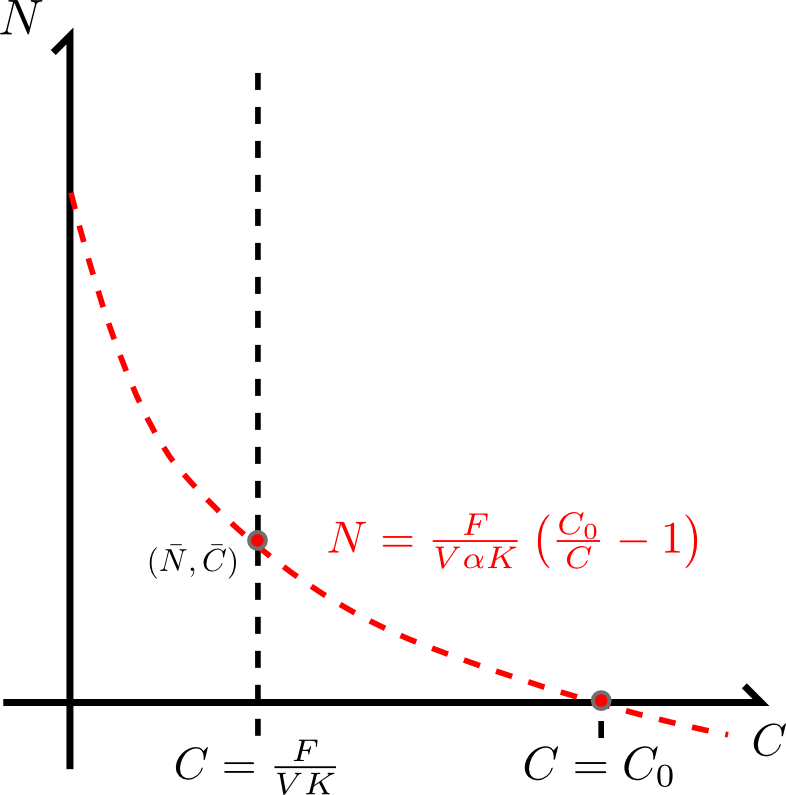
\includegraphics[width=0.35\textwidth]{images/drawing.png}
  \caption{\footnotesize The $\dot{C} = 0$ nullcline (dashed red) intersecting with the $\dot{N} = 0$ nullcline (dashed black).  The trivial and non-trivial steady-states $(0, C_0)$ and $(\bar{N}, \bar{C})$ are shown as red dots.}
\end{figure}
\vfill
\columnbreak
By placing Eq.\ (3) inside Eq.\ (4), we can find the non-trivial steady-state, the intersection of null-clines:
\begin{align}
  \bar{N}(\bar{C}) &= \frac{FC_0}{V \alpha K \bar{C}} - \frac{F}{V \alpha K}  \notag \\
  &= \frac{FC_0}{V \alpha K \frac{F}{VK}} - \frac{F}{V \alpha K} \notag \\
  &= \frac{C_0}{\alpha} - \frac{F}{V \alpha K} = \frac{1}{\alpha} \left( C_0 - \frac{F}{VK} \right).
\end{align}
The unknown parameters in Eq (5) are $\alpha$ and $K$.  We can find these parameters by fitting Eq (5) to the data by non-linear least squares fitting $\bar{N}_i$ at $F_i$ for $i = 1,\ldots,n$, where $n$ is the number of observations.
\end{multicols}

After we obtain estimates of these parameters for both the killer yeast $L$ and sensitive yeast $S$, ($\alpha_L$, $\alpha_S$ and $K_L$, $K_S$ respectively), we can model a ``what if'' scenario whereby we place both species of yeast, sensitive and killer, into one chemostat (assuming the sensitive yeast are resistant to the killer yeast toxin).  The differential equations we use to solve this three-species model is
\begin{align}
  \frac{dL}{dt} &= K_L CL - \frac{FL}{V}, \\
  \frac{dS}{dt} &= K_S CS - \frac{FS}{V}, \\
  \frac{dC}{dt} &= -\alpha_L K_L CL -\alpha_S K_S CS - \frac{FC}{V} + \frac{FC_0}{V}.
\end{align}


The data we are provided with include two sets of two separate runs, along with the concentration of nutrient in the reservoir, $C_0 = 0.02$:
\section{K1 Run}
\subsection*{Vessel One :}
\begin{center}
\begin{tabular}{l|cccccccc}
  Volumes/Hr & 0.028 & 0.099 & 0.142 & 0.207 & 0.269 & 0.287 & 0.352 & 0.403 \\
  Optical Density at Steady State & 0.144 & 0.151 & 0.099 & 0.069 & 0.045 & 0.02 & 0.003 & 0 \\
\end{tabular}
\end{center}

\subsection*{Vessel Two :}
\begin{center}
\begin{tabular}{l|ccccccccc}
  Volumes/Hr & 0.054 & 0.11 & 0.141 & 0.199 & 0.257 & 0.296 & 0.348 & 0.397 & 0.41 \\
  Optical Density at Steady State & 0.164 & 0.151 & 0.11 & 0.092 & 0.072 & 0.023 & 0.006 & 0.002 & 0.004 \\
\end{tabular}
\end{center}

\section{Sensitive Run}
\subsection*{Vessel One :}
\begin{center}
\begin{tabular}{l|ccccccccc}
  Volumes/Hr & 0.041 & 0.099 & 0.167 & 0.223 & 0.266 & 0.328 & 0.356 & 0.401 & 0.462 \\
 Optical Density at Steady State & 0.54 & 0.494 & 0.459 & 0.395 & 0.229 & 0.019 & 0.006 & 0.003 & 0  \\
\end{tabular}
\end{center}

\subsection*{Vessel Two :}
\begin{center}
a\begin{tabular}{l|ccccccc}
 Volumes/Hr & 0.0571 & 0.126 & 0.196 & 0.263 & 0.313 & 0.383  \\
  Optical Density at Steady State & 0.385 & 0.456 & 0.363 & 0.197 & 0.044 & 0.004 \\
\end{tabular}
\end{center}

\begin{figure}[H]
  \centering
    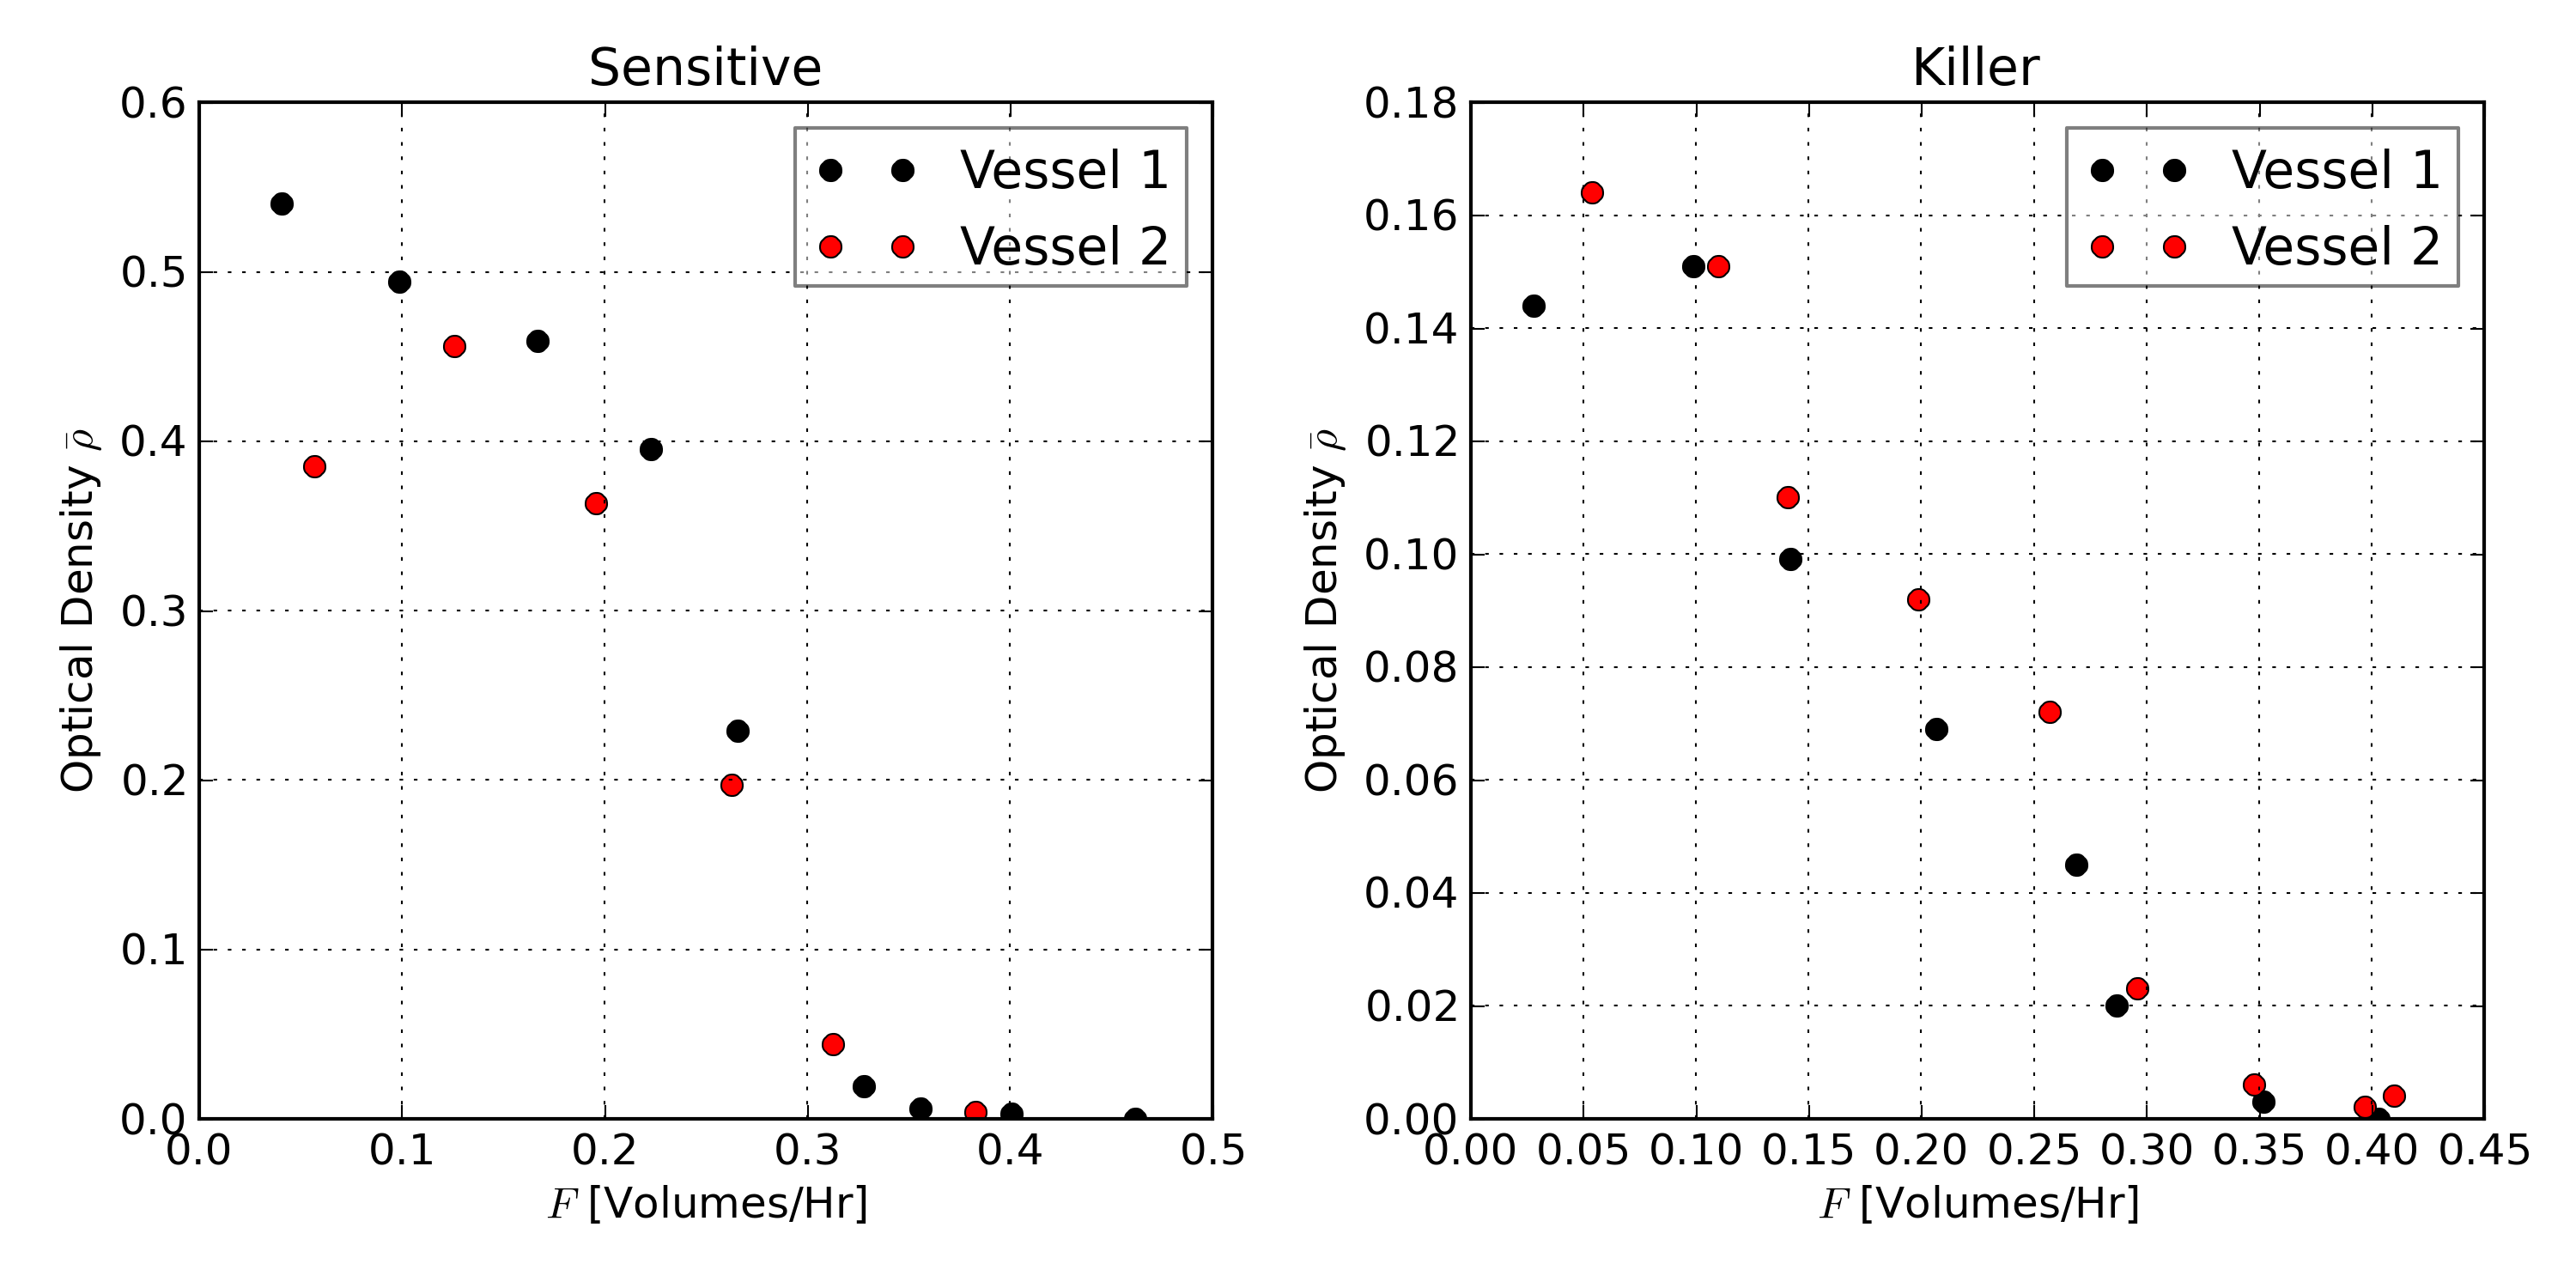
\includegraphics[width=1.0\textwidth]{images/data.png}
\end{figure}

The data provided does not include the volume of the chamber, $V$.  In order to solve Eq.\ (5), this quantity is needed.  Here we have dimensional analysis of the problem:

\begin{align*}
  \frac{dN}{dt} &= KCN - \frac{FN}{V} \\
  \equiv \left[ \frac{1}{\text{time}} \right] &\equiv \left[ \frac{1}{\text{time}} - \frac{\text{volume}}{\text{time}} \cdot \frac{1}{\text{volume}} \right] \equiv \left[ \frac{1}{\text{time}} \right], \\
  \frac{dC}{dt} &= -\alpha KCN - \frac{FC}{V} + \frac{FC_0}{V} \\
  \equiv \left[ \frac{1}{\text{time}} \right] &\equiv \left[ -\frac{1}{\text{time}} - \frac{\text{volume}}{\text{time}} \cdot \frac{1}{\text{volume}} + \frac{\text{volume}}{\text{time}} \cdot \frac{1}{\text{volume}} \right] \equiv \left[ \frac{1}{\text{time}} \right].
\end{align*}

\end{document}


